\documentclass[8.5pt,a4paper]{article}
\usepackage[utf8]{inputenc}
\usepackage[T1]{fontenc}
\usepackage[spanish,es-noshorthands,es-tabla]{babel}
\usepackage{lmodern,microtype,graphicx,booktabs,amsmath}
\usepackage[table]{xcolor}
\usepackage[margin=0.68cm,top=0.45cm,bottom=0.42cm]{geometry}
\usepackage{hyperref}
\definecolor{azul}{HTML}{14334B}
\definecolor{acento}{HTML}{006699}
\definecolor{suave}{HTML}{EAF3F8}
\definecolor{ftsuave}{HTML}{FEF3C7}
\definecolor{ambar}{HTML}{B45309}
\definecolor{gris}{HTML}{4A5560}
\hypersetup{colorlinks=true,urlcolor=acento,linkcolor=acento,pdftitle={Fine-tuning QLoRA del agente Redactor en normativa de pregrado},pdfauthor={Álvaro Contreras y Pablo Cortés},pdflang={es-CL}}
\pagestyle{empty}
\setlength{\parindent}{0pt}
\setlength{\parskip}{1.0pt}
\emergencystretch=1.6em
\newcommand{\seccion}[1]{\par\vspace{1.6pt}{\color{azul}\bfseries\fontsize{8.7}{9.8}\selectfont #1}\par\vspace{0.5pt}}
\newcommand{\sub}{\fontsize{7.45}{8.55}\selectfont}
\newcommand{\REPO}{https://github.com/Pacortes2021/GENERATIVE-ARTIFICIAL-INTELLIGENCE-DELIVERABLE-1/tree/deliverable-4/Deliverable\%204}
\newcommand{\HFURL}{https://huggingface.co/Pablox0333/qwen3-4b-redactor-udec-d4}
\begin{document}
{\color{azul}\bfseries\fontsize{12.2}{13.6}\selectfont Especialización QLoRA del agente Redactor en normativa UdeC}\par
{\color{acento}\bfseries\fontsize{8.5}{9.8}\selectfont Entregable 4 $\cdot$ Fine-tuning supervisado sobre Qwen/Qwen3-4B en arquitectura multi-agente}\par
{\fontsize{7.3}{8.3}\selectfont \textbf{Generative Artificial Intelligence (580694)} $\cdot$ Segundo semestre 2026\hfill Álvaro Contreras y Pablo Cortés}\par
{\fontsize{7.3}{8.3}\selectfont \textbf{Repo:} \href{\REPO}{Deliverable 4 (deliverable-4)} $\cdot$ \textbf{HF:} \href{\HFURL}{Pablox0333/qwen3-4b-redactor-udec-d4} $\cdot$ \textbf{Video ($\leq$3m):} [Pendiente enlace] (\href{\REPO/video}{video/})}\par
\vspace{1.2pt}{\color{azul}\hrule height .62pt}\vspace{1.0pt}

\seccion{1. Continuidad D1--D3, elección empírica del agente y restricción de modelo}
{\sub
Continuamos D1--D3 sobre normativa UdeC (\textbf{197 unidades / 201 fragmentos} de RG, RI-FI y Calendario 2026), embeddings E5, \textbf{75 preguntas oficiales} (50 orig. + 25 dif.) y el grafo de cuatro agentes sobre \textbf{Qwen/Qwen3-4B} ($T=0{,}7$, modo \textit{thinking} OFF). En las trazas D3 v6 (\textbf{66/75}), \textbf{8/9 errores finales (88,9\%)} (\texttt{P13, P24, P26, H07, H14, H18, H25, P36}) ya tenían la evidencia en el \texttt{top-6} del \textbf{Redactor}, además de 11 fallos en primer borrador (\texttt{sin\_verificador}: 63/75) y 25 rechazos hacia ese rol. Ajustar prompts fracasó: en D3 v5 editar \texttt{03\_redactor.txt} bajó 58/75 a 55/75 (revertido a v4), y quitar CoT (\texttt{sin\_cot}: 65/75) casi empató al sistema. Por ello fine-tuneamos solo al \textbf{Redactor}; \texttt{Enrutador}, \texttt{Recuperador} y \texttt{Verificador} conservan pesos base vía \texttt{disable\_adapter()} (548/548 OFF y 100/100 ON en las 75; 182/182 OFF y 30/30 ON en \texttt{nuevas\_20}; \textbf{0 violaciones}, $\max|\Delta\mathrm{logits}|=13{,}56$).}

\seccion{2. Grafo multi-agente con aislamiento LoRA en el Redactor}
\vspace{-2pt}\centerline{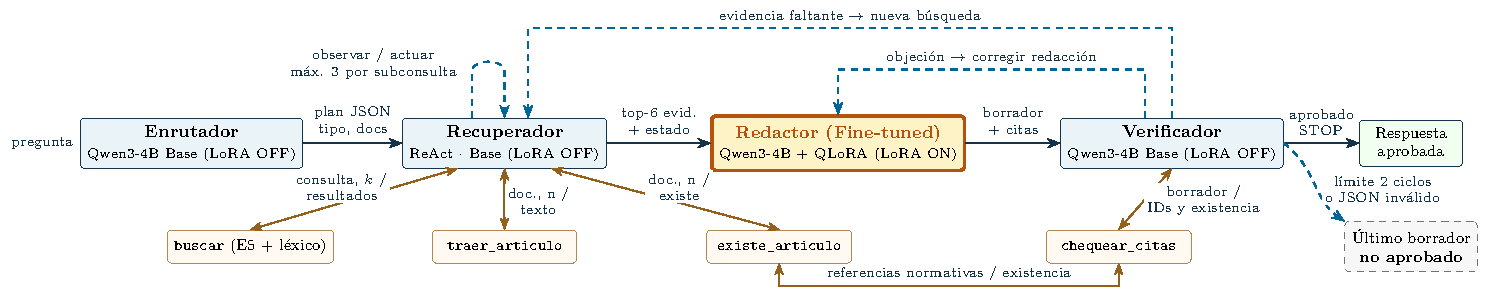
\includegraphics[width=0.92\linewidth]{grafo_d4.pdf}}
\vspace{-2pt}{\fontsize{6.9}{7.9}\selectfont\color{gris} Solo \textbf{\color{ambar}Redactor} carga el adaptador LoRA entrenado; los otros tres roles mantienen pesos base \texttt{Qwen/Qwen3-4B} y prompts \texttt{prompts/01--04} idénticos a D3 v6.}\par
\vspace{1.4pt}{\color{azul!35}\hrule height .4pt}\vspace{1.2pt}

\noindent\begin{minipage}[t]{0.486\linewidth}
\sub\raggedright
\seccion{3. Datos (v2 antifuga), autoría y control de solapamiento}
Construimos \textbf{210 pares híbridos (180 train / 30 val)} en \texttt{redactor\_train.jsonl} y \texttt{redactor\_val.jsonl} bajo el esquema exacto de \texttt{03\_redactor.txt} (\texttt{<pensar>} + \texttt{Respuesta / Condiciones o límites / Fuente}). Cada ejemplo ensambla \textbf{3--6 unidades literales} de \texttt{corpus.json} (mediana 4,0 en v2; \texttt{seed=202604}), cubriendo 112/197 unidades.\par

\textbf{Bloques (train/val):} \texttt{citas\_cruce} (35/5), \texttt{condiciones\_excepciones} (35/5), \texttt{polares\_y\_lectura} (30/5), \texttt{calculos\_y\_orden} (30/5), \texttt{resiliencia\_feedback} (25/5) y \texttt{abstencion\_honesta} (25/5); estados v2: \texttt{suficiente} (189), \texttt{insuficiente} (16) y \texttt{no\_existe} (5).\par

\textbf{Corrección v1$\rightarrow$v2, autoría y auditoría:} En v1 detectamos fuga semántica (0 con \texttt{No aplica} y 4 trazas que nombraban QIDs de eval). En \textbf{dataset v2} imponemos \textbf{0\% solapamiento de unidades} con las 40 unidades de eval D3 y las 21 reservadas de \texttt{preguntas\_nuevas\_20.csv}, \textbf{0 menciones QIDs/trampas} y \textbf{74/210} con \texttt{Condiciones o límites: No aplica}; antifuga léxico marca \textbf{0 alertas} ($\text{seq\_ratio}\ge 0{,}85$, $\text{Jaccard}\ge 0{,}80$). \textbf{Autoría:} pares curados con \textbf{asistencia de IA (Antigravity)} y muestra de 30 casos en \texttt{MUESTRA\_REVISION\_MANUAL.md} (pendiente firma final de par).\par

\seccion{4. Configuración QLoRA y curva de pérdida (corrida v2)}
Entrenamiento QLoRA de \texttt{Qwen/Qwen3-4B} ($\sim$4,0B nominales; 2,24B empaquetados en 4-bit NF4, doble cuantización, \texttt{float16}) en \textbf{Tesla T4 (15,64 GB VRAM)} durante \textbf{52,38 min (90 pasos / 3,0 épocas)}. LoRA $r=16$, $\alpha=32$, \texttt{dropout}=0,05 en 7 proyecciones (\texttt{q,k,v,o,gate,up,down\_proj}: 33,03M entrenables = \textbf{1,48\%} del modelo NF4 / $\sim$0,82\% de 4B), \texttt{batch}=1, \texttt{grad\_accum}=6, \texttt{lr}=$10^{-4}$ coseno (\texttt{warmup}=9), \texttt{paged\_adamw\_8bit} y \texttt{completion\_only\_loss=True}. Sobre v2 (\textbf{0 truncados} a 4096 tokens; max 3395 train / 3354 val), \texttt{eval\_loss} baja de \textbf{1,6006} (paso 0) a \textbf{0,5164} (paso 90), y \texttt{train\_loss} final agregada = \textbf{0,6261}.\par

\vspace{2pt}\centerline{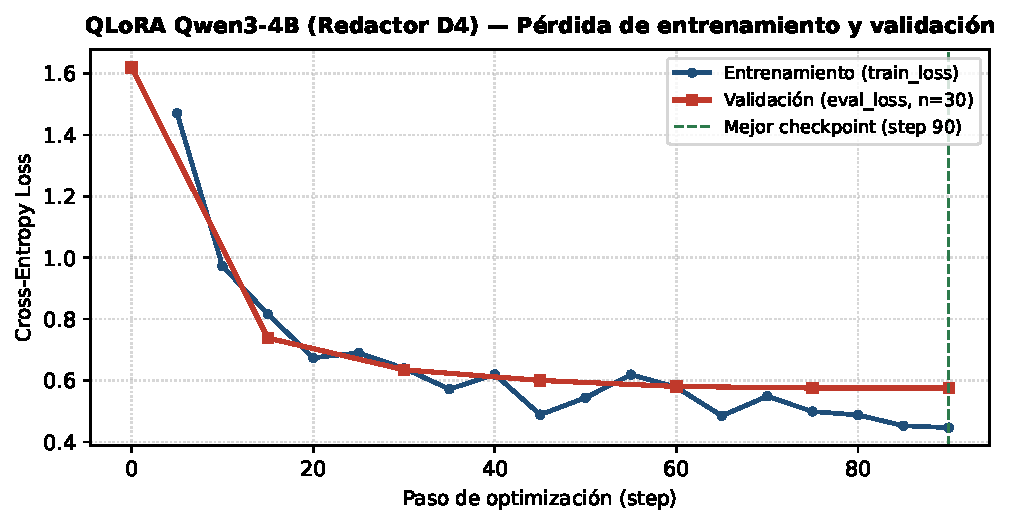
\includegraphics[width=0.92\linewidth]{../entrenamiento/loss_curve.pdf}}
\vspace{-1pt}{\fontsize{6.8}{7.8}\selectfont\color{gris} Adaptador v2 publicado en HF: \texttt{Pablox0333/qwen3-4b-redactor-udec-d4} (\texttt{main}).\par}
\end{minipage}\hfill
\begin{minipage}[t]{0.488\linewidth}
\sub\raggedright
\seccion{5. Resultados v2 (A100 bf16): 75 oficiales, Control y 20 nuevas}
Evaluamos bajo pauta estricta D2/D3 (\texttt{LEEME\_PAUTA.md}, Regla 3 / \texttt{P01}). \textit{Control limpio:} ejecutamos \texttt{Control Base (--solo-base)} y \texttt{Redactor FT v2} en el mismo \textbf{A100 40 GB (\texttt{bf16})}, además del set ciego \texttt{preguntas\_nuevas\_20.csv}.\par

\vspace{1.5pt}
{\fontsize{6.45}{7.5}\selectfont\setlength{\tabcolsep}{1.0pt}
\renewcommand{\arraystretch}{1.04}
\begin{tabular*}{\linewidth}{@{\extracolsep{\fill}}lccccc@{}}
\toprule
\textbf{Sistema} & \textbf{Orig.(50)} & \textbf{Dif.(25)} & \textbf{Tot.(75)} & \textbf{N20} & \textbf{Ll./q}\\
\midrule
D1 Directo (T4) & 1 (2\%) & 0 (0\%) & 1 (1,3\%) & --- & 1,0\\
D2 RAG E5 (T4) & 40 (80\%) & 16 (64\%) & 56 (74,7\%) & --- & 1,0\\
D3 Base (T4) & \textbf{46 (92\%)} & \textbf{20 (80\%)} & \textbf{66 (88,0\%)} & --- & 9,5\\
D4 Base (A100) & \textbf{46 (92\%)} & 16 (64\%) & 62 (82,7\%) & \textbf{11 (55\%)} & 8,8/12,7\\
\rowcolor{ftsuave}\textbf{D4 FT v2 (A100)} & 43 (86\%) & 17 (68\%) & 60 (80,0\%) & 10 (50\%) & \textbf{8,6/10,6}\\
\bottomrule
\end{tabular*}}
\vspace{1pt}{\fontsize{6.6}{7.55}\selectfont\color{gris} N20: \texttt{nuevas\_20}; Ll./q: llamadas/preg. (75 / N20). 0 citas fuera de evidencia y 0 violaciones LoRA. En A100 (\texttt{bf16}): 75 preg. en 75,69 min FT vs 75,34 Base (648 vs 658 llam.; \textbf{$-$8,86\% vs D3} 711); en N20, FT reduce \textbf{$-$16,5\% llam.} (212 vs 254) y \textbf{$-$23,7\% tiempo} (25,07 vs 32,84 min; 1 fallback). Núcleo FT v2 sin \texttt{P01}: 62/75.\par}

\textbf{Avances v1$\rightarrow$v2 y contraste pareado:} Frente a D3 v6, FT v2 corrige \textbf{5/9 fallos de D3} (\texttt{P13, P24, H07, H14, H18}), recupera \textbf{6 errores de v1} (\texttt{P6, P7, P10, P31, H18, H19}) y eleva \texttt{No aplica} de 0/75 a \textbf{37/75} (Base: 12/75) y \textbf{12/20} en \texttt{nuevas\_20} (Base: 0/20). Frente al Control Base A100, FT v2 vence en \textbf{6 casos} (\texttt{P11, P43, H07, H18, H19, H24}), logra \textbf{4/6 vs 2/6} en comparativa pareada D3 (\texttt{H07}: $42/4=10{,}5$ en 2 ciclos / 89,0\,s vs Base abstención 173,5\,s; \texttt{H14} en 1 ciclo) y \textbf{2/3 vs 1/3} en pareada de \texttt{nuevas\_20} (\texttt{N01}). Por categoría vs D3: mejora \texttt{numerica} ($9\rightarrow10$), \texttt{negacion\_excepcion} ($2\rightarrow3$) y \texttt{sintesis} ($3\rightarrow4/5$); cae en \texttt{multi\_salto} ($3\rightarrow1/4$), \texttt{premisa\_falsa} ($4\rightarrow2/4$), \texttt{condicional} ($8\rightarrow7$) y \texttt{factual} ($10\rightarrow8$; 10/10 núcleo).\par

\seccion{6. Fallos v2, Verificador como techo y análisis crítico}
Auditoría de los \textbf{15 fallos en 75} y \textbf{10 en \texttt{nuevas\_20}} (\texttt{casos\_fallo\_y\_regresion.json}):\par

\textbf{1) \texttt{Verificador} base degrada borradores válidos (\texttt{H04, H06, H21, H22, N05}):} En \textbf{5 casos}, \texttt{Redactor FT v2} acierta en ciclo 1 (\texttt{38/4=9,5} en \texttt{H06}, \texttt{4,0} en \texttt{H22}, \texttt{[RG-ART-049]} en \texttt{H04}, mínimo 8 en \texttt{H21}, Art.\,6 en \texttt{N05}), pero el \texttt{Verificador} (\texttt{disable\_adapter()}) rechaza el borrador e induce fallos en ciclos 2--3. En 75, \textbf{12/68} aprobaciones fallan y \textbf{4 de 7 rechazos} recaen en respuestas válidas (\texttt{P38, P47, P48, P50}).\par

\textbf{2) Cuellos en \texttt{Recuperador} y \texttt{Enrutador} base (\texttt{H03, N12, N19}):} \texttt{CAL-2026-S2-02} sigue fuera del \texttt{top-6} en \texttt{H03} (ambos fallan); en \texttt{nuevas\_20}, \texttt{Enrutador} filtra solo \texttt{RI-FI} excluyendo \texttt{RG} en \texttt{N12} (0 fuentes) y \texttt{N19}.\par

\textbf{3) Errores residuales del Redactor:} \texttt{No aplica} omite excepciones (\texttt{P36, H25}); alucinación \textit{``simulink''} sin \texttt{Fuente:} (\texttt{H02}); aritmética de fechas en \texttt{N06, N07}; mezcla de plazos (\texttt{H12, P26, P28}); desvíos \texttt{P01}/lectura (\texttt{P5, P8, P25, P45, N08, N10, N16--N18}). Limitar LoRA al Redactor deja al \texttt{Verificador} base como principal cuello de botella.\par

\seccion{7. Reproducibilidad}
En \texttt{Deliverable 4/}: \texttt{scripts/} (\texttt{construir\_dataset.py}, \texttt{entrenar\_redactor.py}, \texttt{evaluar\_d4.py} con \texttt{--solo-base} y \texttt{--preguntas-csv}, \texttt{generar\_auditoria\_d4.py}), prompts \texttt{prompts/01--04}, \texttt{datos/preguntas\_nuevas\_20.csv}, métricas/trazas v2 y guía en vivo en \texttt{video/}.\par
\end{minipage}
\end{document}
